\chapter{Experiences}
\label{sec:experiences}

\section{Samples}

Sample characterization


\section{Uncovering important variables}


\subsection{Feature importance with RandomForestClassifier}

The following experiments were designed using the RandomForestClassifier algorithm \cite{scikit-learn}. The goal was to obtain important features that would be able to explain the occurrence of wildfires. These tests were conducted on the three samples previously mentioned.

Firstly, for each sample, a wildfire occurrence was set 3 hours before the wildfire occurrence and 1 hour after, and then the most important variables were calculated. Their complete hourly records were used. With a random state of 445621151 for RandomForestClassifier, the tables \ref{importance_2015_2019} and \ref{importance_2022} show the results for each year.

\begin{table}[H]
	\caption{Variable importance for 2015 and 2019}
	\label{importance_2015_2019}
	\centering
	\begin{tabular}{llll}
		\multicolumn{1}{|l}{2015}      & \multicolumn{1}{l|}{} & 2019                              & \multicolumn{1}{l|}{} \\ \hline
		Variable                       & Importance            & Variable                          & Importance            \\
		soil\_moisture\_100\_to\_255cm & 0.122                 & wind\_speed\_100m                 & 0.072                 \\
		DMC                            & 0.057                 & soil\_temperature\_100\_to\_255cm & 0.065                 \\
		ISI                            & 0.053                 & BUI                               & 0.062                 \\
		BUI                            & 0.051                 & soil\_temperature\_7\_to\_28cm    & 0.056                 \\
		wind\_speed\_100m              & 0.042                 & soil\_moisture\_100\_to\_255cm    & 0.053                
	\end{tabular}
\end{table}

\begin{table}[H]
	\caption{Variable importance for 2022}
	\label{importance_2022}
	\centering
	\begin{tabular}{ll}
		\hline
		2022     &            \\ \hline
		Variable & Importance \\
		DMC      & 0.127      \\
		BUI      & 0.111      \\
		DC       & 0.087      \\
		ISI      & 0.054      \\
		FWI      & 0.052     
	\end{tabular}
\end{table}

The last 24 rows of each sample were assigned as 1 in the boolean scale of wildfire occurrence, while the rest were assigned as 0. With the RandomForestClassifier algorithm, it was possible to obtain the data shown in Table \ref{hourly_values} depicting the five most important features according to this method.
The two least important features are \textit{rain} and \textit{precipitation}. Although \textit{rain} was considered one of the least important features, it cannot be discarded because it is a variable in \textit{FWI} component analysis, and three components from \textit{FWI} are among the most important features that appear in table \ref{hourly_values}.

\begin{table}[H]
	\caption{Variable importance for hourly values}
	\centering
	\label{hourly_values}
	\begin{tabular}{lc}
		\hline
		Variable                       & \multicolumn{1}{l}{Importance} \\ \hline
		DC                             & 0.091                          \\
		DMC                            & 0.075                          \\
		soil\_moisture\_100\_to\_255cm & 0.073                          \\
		BUI                            & 0.067                          \\
		surface\_pressure              & 0.067                         
	\end{tabular}
\end{table}


Table \ref{daily_values} displays the five most important features, according to a daily average value. For each variable, a mean value was calculated, and it was assigned to the last day as a boolean value for wildfire 1, depicting an occurrence of a wildfire. This method showed little improvement in relation to the one shown in table \ref{hourly_values}. The two least important features considered were \textit{precipitation} and \textit{dew\_point\_2m}.
\begin{table}[H]
	\caption{Variable importance with daily mean method}
	\centering
	\label{daily_values}
	\begin{tabular}{lc}
		\hline
		Variable                        & \multicolumn{1}{l}{Importance} \\ \hline
		soil\_moisture\_100\_to\_255cm  & 0.100                          \\
		soil\_moisture\_28\_to\_100cm   & 0.090                          \\
		terrestrial\_radiation          & 0.075                          \\
		wind\_speed\_100m               & 0.072                          \\
		terrestrial\_radiation\_instant & 0.054                         
	\end{tabular}
\end{table}


Another experiment was conducted by selecting a time frame between 9:00 and 20:00 hours. Taking a glace at figure \ref{fig:daily_fwix_2015_2019_2020}, the value of \textit{FWI} starts to increase around 8 or 9 in the morning, has its highest value around 15, and then it starts to decrease. After around 20 hours, it reaches its lowest point in the samples from the years 2015 and 2019. 


Table \ref{hourly_importance_fwix_2015_2019_2020} shows soil moisture as the most important feature, like in Table \ref{hourly_values}. There was also another experiment where the time frame was selected according to the hour of the wildfire. 


\begin{figure}[h]
	\centering
	\caption{Hourly FWI value for the day of wildfire occurence}
	\begin{subfigure}{0.45\textwidth}
		\centering
		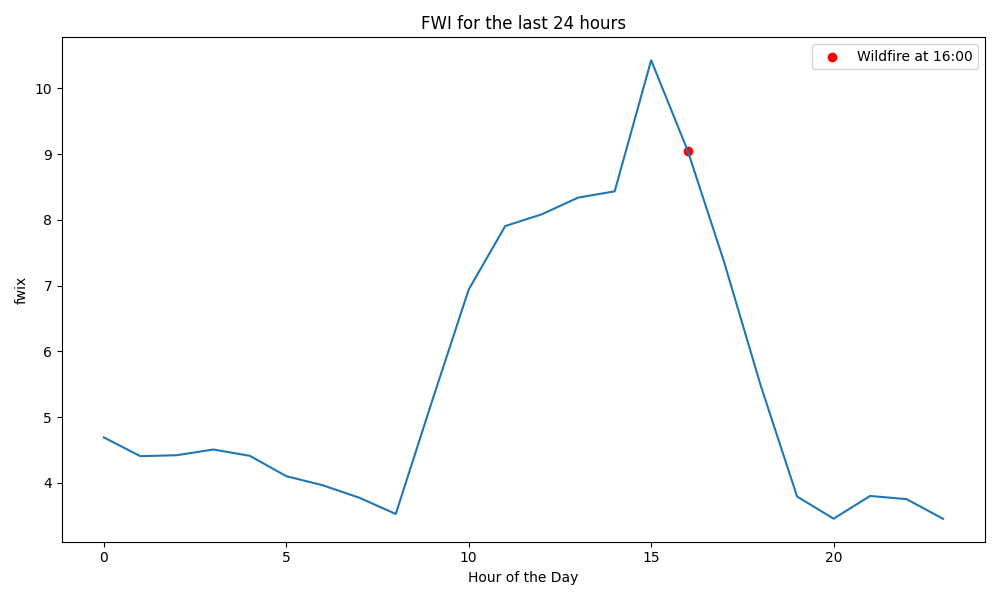
\includegraphics[width=\textwidth]{graphs/variables/fwix_24_2015.png}
		\caption{2015}
	\end{subfigure}
	\hfill
	\begin{subfigure}{0.45\textwidth}
		\centering
		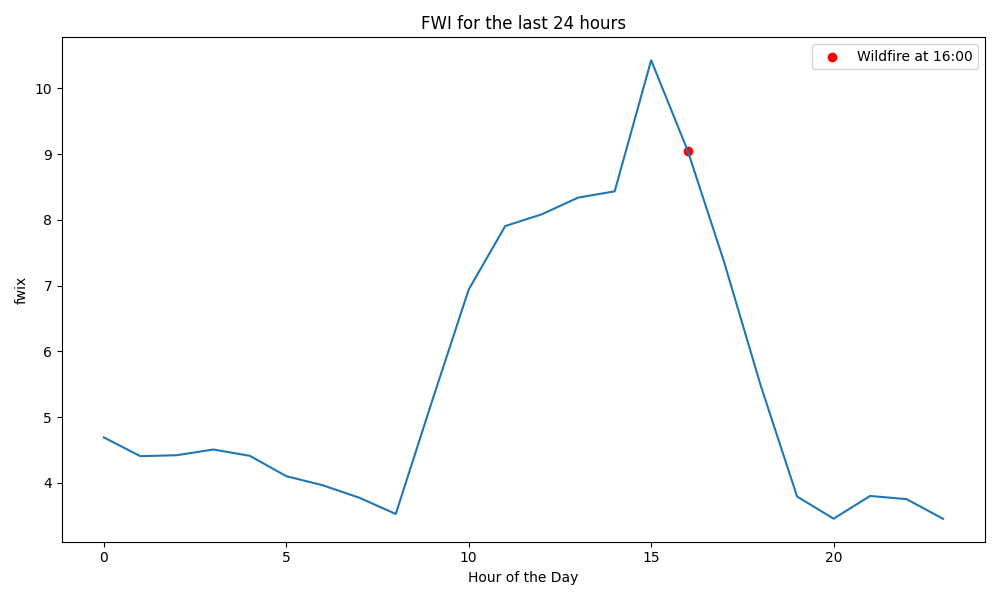
\includegraphics[width=\textwidth]{graphs/variables/fwix_24_2015.png}
		\caption{2019}
	\end{subfigure}
	\hfill
	\begin{subfigure}{0.45\textwidth}
		\centering
		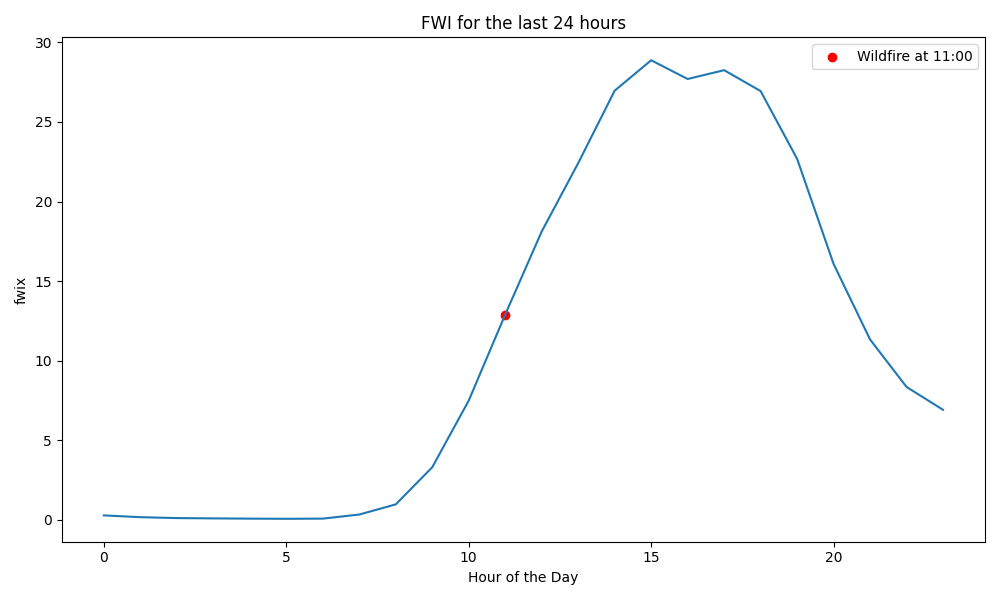
\includegraphics[width=\textwidth]{graphs/variables/fwix_24_2019.png}
		\caption{2022}
	\end{subfigure}
	
	\label{fig:daily_fwix_2015_2019_2020}
\end{figure}

\begin{table}[H]
	\centering
	\caption{Variable importance with \textit{FWI} time frame method}
	\begin{tabular}{lc}
		\hline
		Variable                       & \multicolumn{1}{l}{Importance} \\ \hline
		soil\_moisture\_100\_to\_255cm & 0.072                          \\
		BUI                            & 0.067                          \\
		DC                             & 0.059                          \\
		soil\_moisture\_7\_to\_28cm    & 0.057                          \\
		DMC                            & 0.054                         
	\end{tabular}
	\label{hourly_importance_fwix_2015_2019_2020}
\end{table}

A time frame three hours after and before the hour of wildfire (table \ref{hourly_importance_fwix_2015_2019_2020_3hours}) was selected. It yielded the same variables as table \ref{hourly_importance_fwix_2015_2019_2020} but in a different order.

\begin{table}[H]
	\centering
	\caption{Variable importance with 3-hours time frame method}
	\begin{tabular}{lc}
		\hline
		Variable                       & \multicolumn{1}{l}{Importance} \\ \hline
		DC & 0.073                          \\
		DMC                            & 0.055                          \\
		soil\_moisture\_100\_to\_255cm                             & 0.046                          \\
		soil\_moisture\_28\_to\_100cm    & 0.045                          \\
		BUI                            & 0.043                         
	\end{tabular}
	\label{hourly_importance_fwix_2015_2019_2020_3hours}
\end{table}


The authors from \cite{wang2023improving} set that the maximum time frame for wildfire weather variable analysis is 16 days. Given that the sample from 2022 only contains hourly data for 14 days, the table \ref{14_days_prior_importance} displays the most important features taken 14 days prior to the wildfire occurrence from all three samples. Like the experiment displayed in table \ref{daily_values}, a daily average was calculated for each day.

\begin{table}[H]
	\centering
	\caption{Variable importance 14-days prior time frame method}
	\begin{tabular}{lc}
		\hline
		Variable                         & \multicolumn{1}{l}{Importance} \\ \hline
		soil\_temperature\_28\_to\_100cm & 0.123                          \\
		wind\_speed\_10m                 & 0.105                          \\
		apparent\_temperature            & 0.087                          \\
		terrestrial\_radiation           & 0.072                          \\
		soil\_moisture\_100\_to\_255cm   & 0.049                         
	\end{tabular}
	\label{14_days_prior_importance}
\end{table}

A last experiment (table \ref{14_days_prior_hourly_importance}) was also conducted with an hourly method. The last 360 rows from each sample were selected without taking in averages, it was set as a boolen variable for wildfire occurrence all rows 3 hours prior and 2 hours after the wildfire. 

\begin{table}[H]
	\centering
	\caption{Variable importance 14-days prior hourly time frame method}
	\begin{tabular}{lc}
		\hline
		Variable                         & \multicolumn{1}{l}{Importance} \\ \hline
		sunshine\_duration & 0.125                          \\
		apparent\_temperature                 & 0.111                          \\
		soil\_temperature\_0\_to\_7cm            & 0.107                          \\
		temperature\_2m           & 0.107                          \\
		terrestrial\_radiation   & 0.100                         
	\end{tabular}
	\label{14_days_prior_hourly_importance}
\end{table}


